\section{Text-to-Tree transformation}

As we shall see in a moment, libraries and shelves correspond to a folder structure while the contents for a single dictionary are specified in a file.
Figure \ref{fig:moca-4-Tokens} depicts a small sample of the textual syntax used to specify a dictionary.
On the way to an instance model of our dictionary metamodel, the very first step is to create nice \emph{chunks} of characters.
This step is called \emph{lexing} and it simplifies the actual comprehension of the complete text.
Interestingly human beings actually comprehend text in a similar manner, one recognizes whole words without ``seeing'' every individual character.
This is the reason why you can siltl raed tihs sneentce alsomt eforftlsesly.   
A lexer recognizes these chunks or \emph{tokens} and passes them on as a token stream to the \emph{parser} that does the actual work of recognizing complex hierarchical and recursive structures.   
   
To recognize the tokens as indicated in Fig.~\ref{fig:moca-4-Tokens}, \texttt{ANTLR} can automatically generate a lexer in Java from a compact specification as depicted in Fig.~\ref{fig:moca-6-lexer}.
This is actually a DSL for lexing and is explained in detail in \cite{ANTLR}.
If you do not know what EBNF is and have problems understanding the lexer grammar then make sure you at least go through the documentation on \url{www.antlr.org} or read relevant chapters in \cite{ANTLR}.

%\usepackage{graphics} is needed for \includegraphics
\begin{figure}[!htbp]
\begin{center}
 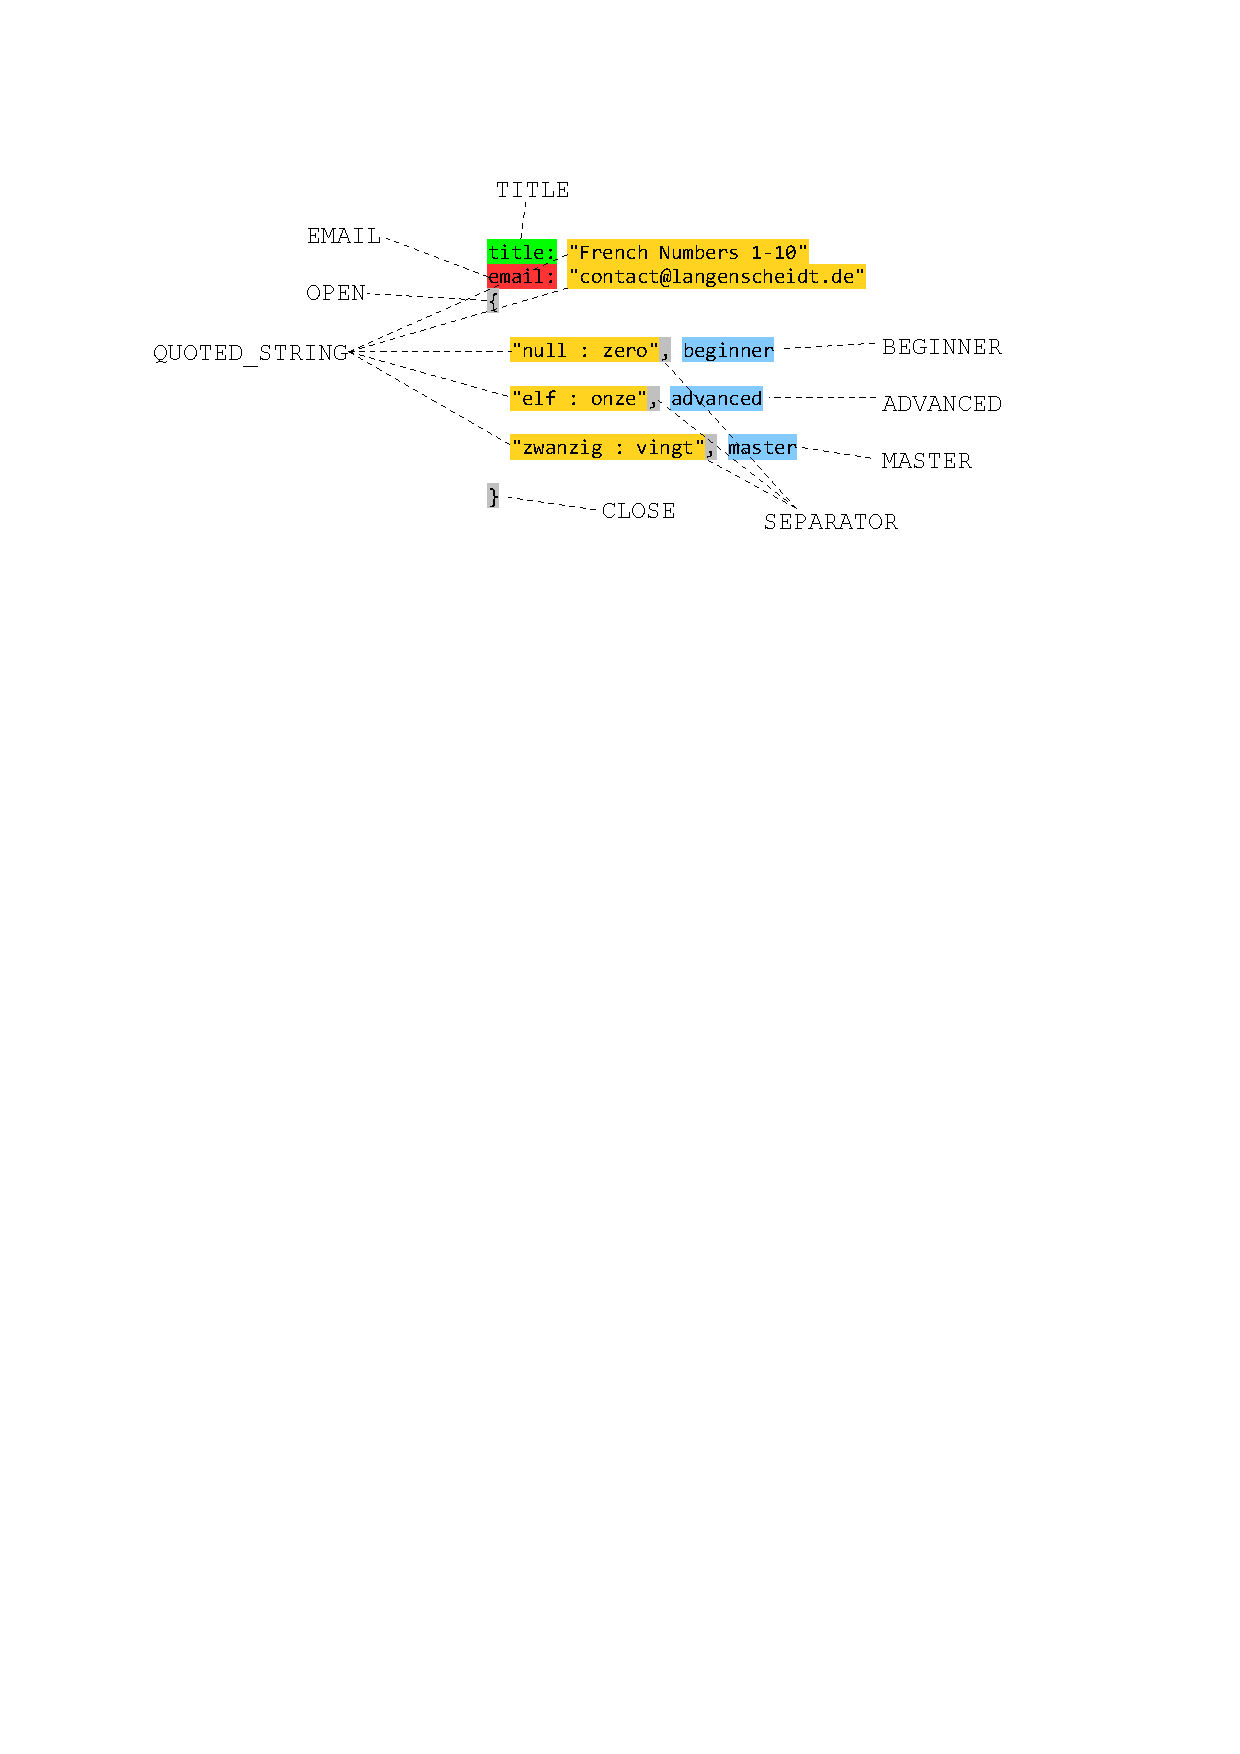
\includegraphics[width=0.7\textwidth]{pics/moca/2TextToMocaTree/4-tokens}
  \caption{Identified tokens in a dictionary file.}
  \label{fig:moca-4-Tokens}
\end{center}
\end{figure}

\begin{enumerate}
\item[$\blacktriangleright$] Edit \texttt{DictionaryLexer.g} so it closely resembles Fig.~\ref{fig:moca-6-lexer}.
Be careful to avoid any typos and mistakes.  Save and make sure it compiles.  
\end{enumerate}

%\usepackage{graphics} is needed for \includegraphics
\begin{figure}[!htbp]
\begin{center}
 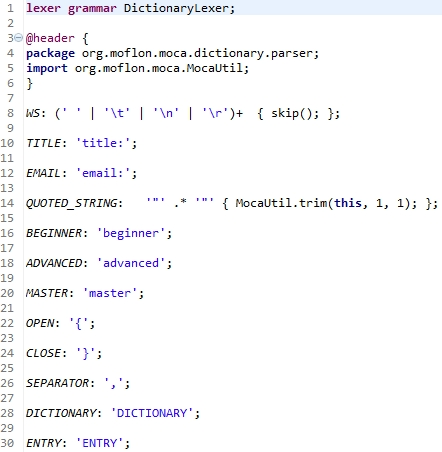
\includegraphics[width=0.65\textwidth]{pics/moca/2TextToMocaTree/6-lexer}
  \caption{Lexer grammar}
  \label{fig:moca-6-lexer}
\end{center}
\end{figure}

The next step is to form the stream of tokens from the lexer into a \emph{tree}.
In this context, a tree is an acyclic, hierarchical, recursive structure as depicted in Fig.~\ref{fig:moca-5-Tree}.
Depending on what the tree is to be used for, it can be organized very differently with extra \emph{structural} nodes like \texttt{DICTIONARY} or \texttt{ENTRY} that were not present in the textual syntax and are used to give additional meaning to the tree. 

%\usepackage{graphics} is needed for \includegraphics
\begin{figure}[htp]
\begin{center}
 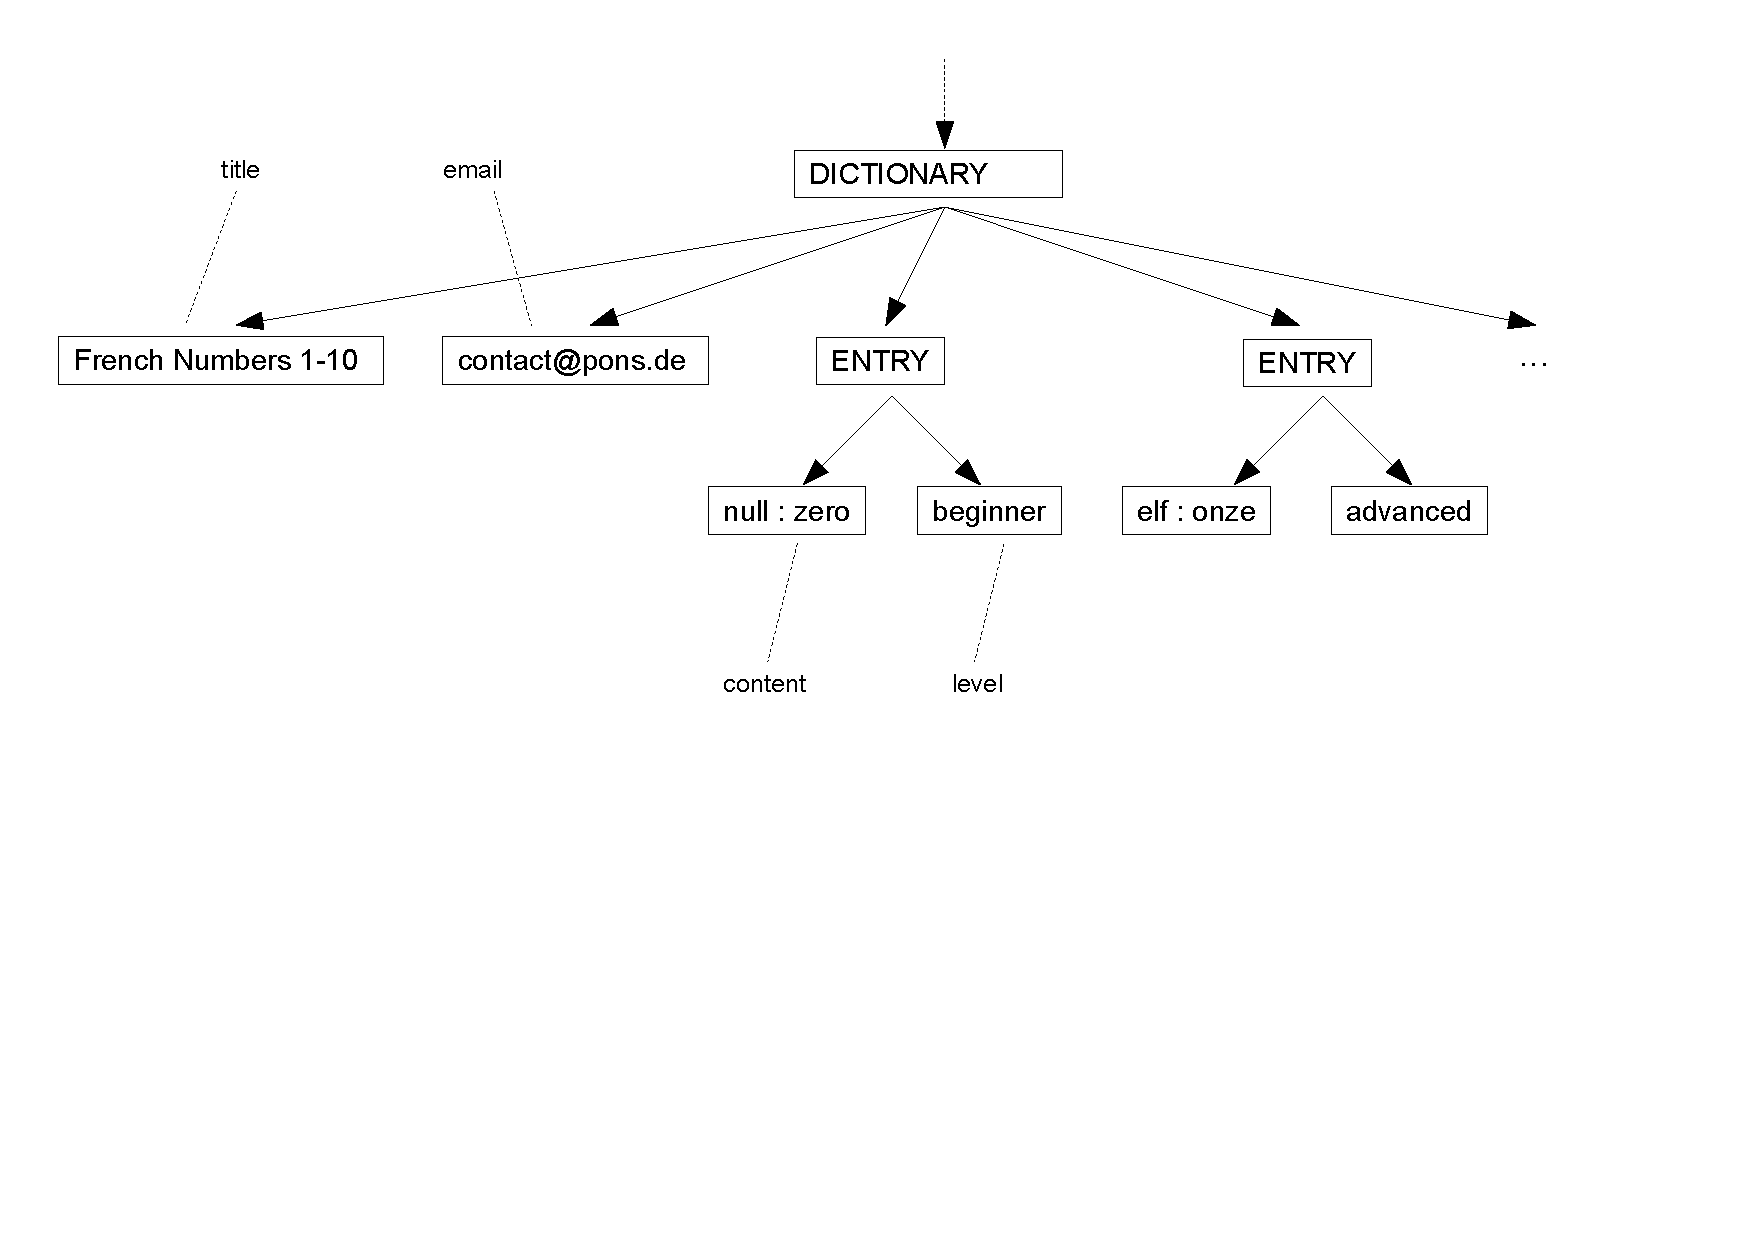
\includegraphics[width=\textwidth]{pics/moca/2TextToMocaTree/5-tree}
  \caption{MocaTree structure}
  \label{fig:moca-5-Tree}
\end{center}
\end{figure}

\begin{enumerate}
\item[$\blacktriangleright$] Edit \texttt{DictionaryParser.g} so it closely resembles Fig.~\ref{fig:moca-7-parser}.
As with the lexer, avoid typos and mistakes and make sure it compiles.
\end{enumerate}

%\usepackage{graphics} is needed for \includegraphics
\begin{figure}[!htbp]
\begin{center}
 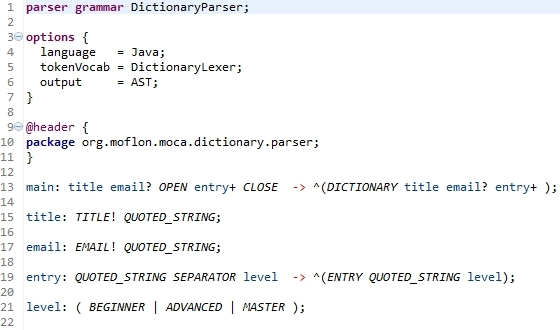
\includegraphics[width=0.9\textwidth]{pics/moca/2TextToMocaTree/7-parser}
  \caption{Parser grammar}
  \label{fig:moca-7-parser}
\end{center}
\end{figure}
The parser grammar is quite similar to the lexer grammar, but there are \emph{parser actions} after the \texttt{->} symbol, which build up the tree.
Using this simple tree language, one can (1) abstract from tokens like \texttt{\{} or \texttt{\}}, which are just \emph{syntactical noise}\footnote{In this context, content that is irrelevant for our model.} and (2) enrich the tree with structural nodes like \texttt{ENTRY}, which add explicit structure to the tree.
Please refer to \cite{ANTLR} and online resources for a detailed explanation of the syntax and semantics of the parser grammar supported by \texttt{ANTLR}. 
 
%\usepackage{graphics} is needed for \includegraphics
\begin{figure}[htp]
\begin{center}
 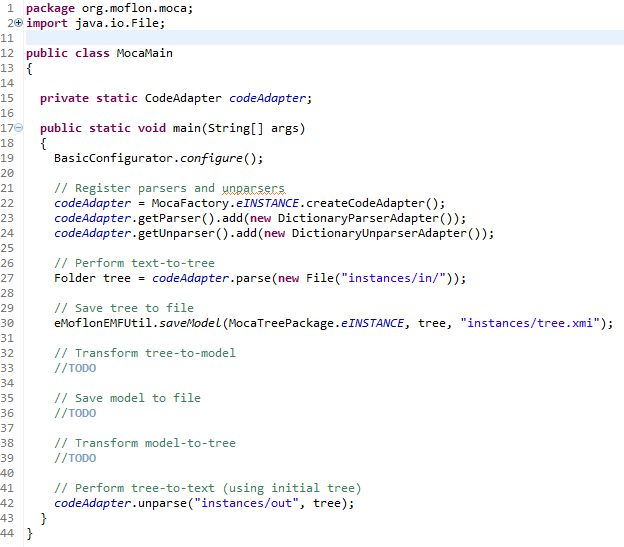
\includegraphics[width=\textwidth]{pics/moca/2TextToMocaTree/8-MocaMain}
  \caption{Generated main method}
  \label{fig:moca-8-MocaMain} 
\end{center}
\end{figure}

Before we take our lexer and parser for a spin, open \texttt{MocaMain.java} and inspect it.
If everything went right it should bear a striking resemblance to Fig.~\ref{fig:moca-8-MocaMain}.
For the moment, please comment out line 24\footnote{If you forget this the default implementation of the unparser will throw an exception.} as we shall define the unparser, i.e., model-to-text a bit later.
Do not change anything else and just note how the parser is added to the Moca framework (line 23) via an adapter (\texttt{Dictionary\-Parser\-Adapter}).
Go ahead and look at what the adapter exactly does.
All the code can be adjusted and used, for example, to define which files the parser is to be used for (per default the adapter registers for \texttt{*.dictionary} files).
The main job of the adapter is to hide \texttt{ANTLR} specifics so the framework remains (parser) technology agnostic.
If you decide to use a different parser generator or write the parser by hand you would need to implement a corresponding adapter from scratch.

On line 27, the input for the framework is set, meaning that all folders in \texttt{./instances/in} are parsed.
In a nutshell, each folder is taken as a root of a tree and the folder and file structure is reflected as a hierarchy of (children) nodes in the tree.
For each file, the framework searches for a registered parser that is responsible for the particular file, passes the content on to the parser and plugs in the tree from the parser as a single subtree of the corresponding file node in the overall tree.  Take a look at Fig.~\ref{fig:moca-overview} again and review the parts we have covered.

The final step is now to prepare some input for the framework:
\begin{enumerate}
  \item[$\blacktriangleright$] Create the directory structure depicted in Fig.~\ref{fig:moca-inputdata} in \texttt{Dictionary\-Code\-Adapter} and enter the contents from Table~\ref{moca-inputdata} for each of the four \texttt{dictionary} files\footnote{You can just copy\&paste right from this PDF file}.
  %\usepackage{graphics} is needed for \includegraphics
\begin{figure}[htp]
\begin{center}
  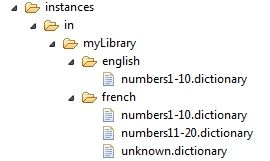
\includegraphics[width=0.5\textwidth]{pics/moca/2TextToMocaTree/inputData}
  \caption{Input directory structure.}
  \label{fig:moca-inputdata}
\end{center}
\end{figure}

\begin{table}
\begin{tabular}{p{6cm} p{6cm} }
\footnotesize
\textbf{english/numbers1-10.dictionary:}
\begin{verbatim}
title: "English Numbers 1-10"
email: "contact@langenscheidt.de"	
{
  "null : zero", beginner
  "eins : one", beginner
  "zwei : two", beginner
  "drei : three", beginner
  "vier : four", beginner
  "fuenf : five", beginner
  "sechs : six", beginner
  "sieben : seven", beginner
  "acht : eight", beginner
  "neun : nine", beginner
  "zehn : ten", beginner 
}
\end{verbatim} 

\textbf{french/numbers1-10.dictionary:}
\begin{verbatim}   
title: "French Numbers 1-10"
email: "contact@pons.de"	
{
  "null : zero", beginner
  "eins : un/une", beginner
  "zwei : deux", beginner
  "drei : trois", beginner
  "vier : quatre", beginner
  "fuenf : cinq", beginner
  "sechs : six", beginner
  "sieben : sept", beginner
  "acht : huit", beginner
  "neun : neuf", beginner
  "zehn : dix", beginner 
}
\end{verbatim}
&

\footnotesize
\textbf{french/numbers11-20.dictionary:}
\begin{verbatim}
title: "French Numbers 11-20"
email: "contact@pons.de"	
{
  "elf : onze", advanced
  "zwoelf : douze", advanced
  "dreizehn : treize", advanced
  "vierzehn : quatorze", advanced
  "fuenfzehn : quinze", advanced
  "sechzehn : seize", master
  "siebzehn : dix-sept", master
  "achtzehn : dix-huit", master
  "neunzehn : dix-neuf", master
  "zwanzig : vingt", master
}

\end{verbatim}
\textbf{french/unknown.dictionary:}
\begin{verbatim}
title: "unknown"
{
  "unbekannt", beginner
}
\end{verbatim}
  \\
\end{tabular}   
\caption{Input files containing dictionaries.}
\label{moca-inputdata}

\end{table}   

\item[$\blacktriangleright$] After creating all the dictionaries, run \texttt{MocaMain.java} as a normal Java application. 
If everything works out right, a file called \texttt{tree.xmi} and an \texttt{out} folder should be created in the \texttt{instances} directory\footnote{You probably have to refresh the \texttt{instances} folder to see the newly created files.}.  
Inspect their contents and compare them to Fig.~\ref{fig:moca-9-ParseResult1}. 
The unparsed files are obviously empty as we haven't implemented an \emph{unparser} yet.  
Don't be irritated by the fact that an \texttt{out/in} is created, this can all be configured in \texttt{MocaMain} but the default assumes \texttt{in} contains multiple folders -- in our case libraries -- and it is therefore treated as the root of the tree.  
One could also unparse directly in \texttt{instances} but the unparsed \texttt{in} would have to be renamed in \texttt{MocaMain}.
\end{enumerate}

%\usepackage{graphics} is needed for \includegraphics
\begin{figure}[!htbp]
\begin{center}
 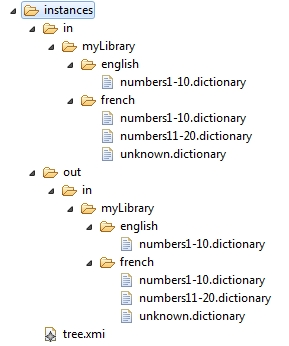
\includegraphics[width=0.4\textwidth]{pics/moca/2TextToMocaTree/9-ParseResult1}
  \caption{Directory \texttt{instances} after parsing}
  \label{fig:moca-9-ParseResult1}
\end{center}
\end{figure} 

\begin{enumerate}
  \item[$\blacktriangleright$] Double-click \texttt{tree.xmi}\footnote{Depending on the plugins you have installed, you might have to explicitly choose \texttt{Open With/Sample Reflective Ecore Model Editor}.} and compare the contents to Fig.~\ref{fig:moca-10-ParseResult2}. At this point, you can reflect on the structure of the tree and note the directory structure, file nodes and the subtrees from the parser.
  
This is important to understand; the directory structure is transformed to a corresponding hierarchy of \texttt{Folders} and \texttt{Files}.
The actual \emph{textual content} of each file is then transformed to a subtree using a registered, suitable parser.
The resulting subtree from the parser is then plugged into the tree by setting its root as the single child node of a \texttt{File}.
%\usepackage{graphics} is needed for \includegraphics
\begin{figure}[!htbp]
\begin{center}
 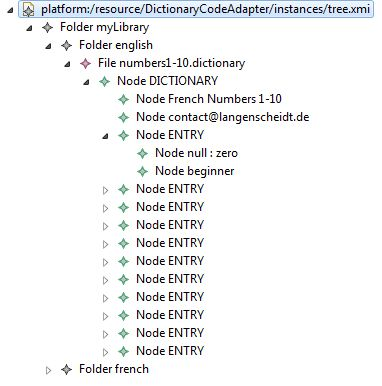
\includegraphics[width=0.55\textwidth]{pics/moca/2TextToMocaTree/10-ParseResult2}
  \caption{MocaTree created by the framework using our parser}
  \label{fig:moca-10-ParseResult2}
\end{center}
\end{figure}
\end{enumerate}

If everything worked out then well done!  We now have a nice tree that we can work on with SDMs and transform in a few simple steps to an actual instance of our Dictionary metamodel.